\documentclass{memoir}
\usepackage{pgfplots}
\usepackage{multicol}
\usepackage{tikz}
\usepackage{amsmath,amssymb}
\usepackage{listings}
\usepackage{color}
\usepackage{caption}
\usepackage[babel=hyphen,backend=biber,citestyle=authoryear]{biblatex}

\addbibresource{PPSources.bib}

\title{ML for HS}
\author{Aidan Sciortino}
\date{March 2017}

%---Custom Colors---%
\definecolor{light-gray}{gray}{0.85}

%---Code Style Template---%
\lstdefinestyle{customj}{
    backgroundcolor=\color{light-gray},
    belowcaptionskip=1\baselineskip,
    breaklines=true,
    frame=L,
    xleftmargin=\parindent,
    language=Java,
    showstringspaces=false,
    basicstyle=\ttfamily,
    keywordstyle=\bfseries\color{green!40!black},
    commentstyle=\itshape\color{purple!40!black},
    identifierstyle=\color{blue},
    stringstyle=\color{orange},
    numbers = left,
}
\lstset{style=customj}

%--Custom Graph Style--%
\pgfplotsset{plot/.style={height=5cm,width=0.5\textwidth,axis lines= middle, axis line style = <->, >=latex,tick align = center,legend style={legend pos = south east, font = \tiny}}}

%---Custom Math Commands---%
\newcommand{\ddx}{ \frac{d}{dx} }
\newcommand{\e}{\text{e}}

%---Neural Network Diagram Shapes---%
\tikzstyle{neuron} = [circle, minimum width= 0.5cm, draw = black]
\tikzstyle{arrow} = [->,>=stealth]
\usetikzlibrary{shapes.geometric, arrows}

\begin{document}
\pagenumbering{roman}

\tableofcontents
\listoffigures

\chapter*{Introduction}
\markboth{Introduction}{Introduction}
  This book was written in response to the lack of resources regarding machine learning designed for those without math backgrounds, or those without the knowledge of the mathematics ``needed'' to fully learn it.

  I have found that the machine learning tutorials, papers, and information online divide themselves into two camps, either;
  \begin{itemize}
    \item \textbf{Over Simplified:} These resources simply apply pre-existing algorithms to data sets, explaining the code behind it but not the mathematics. These are great for people in the industry who simply need an algorithm, but from the perspective of someone trying to learn are very frustrating because they gloss over a lot of material.
    \item \textbf{Over Complicated: } These resources assume a CS or Mathematics background, and therefore don't explain the semantics of the math behind the algorithms. I'm sure that these are great for scientists to read, but from the perspective of a high schooler they are dense, difficult to read, and frustrating to try and understand.
\end{itemize}

  My frustration with these resources led me bite the bullet and learn some complex math in order to better understand both types of resource. However, I decided that I didn't want other people to have to go through what I did, so writing a book seemed logical.

  \subsection{Who This Book is For:}
    This book is designed for students who haven't taken courses in higher math, programmers who want to get into the mechanics behind machine learning but don't have the math knowledge, and anyone who wants to learn more about the fascinating field that is machine learning.

  \subsection{Who This Book (probably) isn't For:}
    People who already have backgrounds in mathematics involving linear algebra, multivariate calculus, advanced statistics, etc. I go into lots of detail about the mathematics behind machine learning that would probably prove boring to most of you.

  \subsection{License}
    Throughout the course of researching, writing, typesetting and coding this book, I have made use of resources that were Creative Commons and Open Source. As a result, you are free to reuse any code examples from this book and sample the text in any way, as long as it isn't for profit. Attribution would be nice but is not required. An email including a link to your project would also be awesome, but again, not required.

    \vspace{0.5em}

In this book I have endeavored to explain every bit of code, every line of math, and every letter of vocabulary. I hope you find it informative, helpful, and interesting.
  \begin{flushright}\emph{-Aidan Sciortino, 2017}\end{flushright}

\chapter{Beginning Neural Networks}
\pagenumbering{arabic}
In this chapter we will build a single layer feed forward neural network using some simple math concepts and an older model called the perceptron. This all may sound complicating at first, but we will break it down into simple parts that can be easily digested.
\section{Objective}
This chapter is designed to serve as an introduction to the mathematics, models, history and logic behind neural networks. The chapter is divided into four sections; one serving as an introduction to the theory behind machine learning, another dedicated to the mathematics needed for this chapter, another explaining some history behind the algorithms used in this chapter, and a last dedicated to the actual code with accompanying explanations.

The chapter is not necessarily designed to be read in order. Readers who believe that they can pick up most of the mathematics and algorithms from reading the code section could skip to there, and then perhaps look back at the mathematics and algorithms sections.
\clearpage

\section{Theory}
Machine learning operates on the principle of modifying input data to return certain output data. For example, we might have the following input data:
\[
	\begin{bmatrix}
		0 & 1 & 0 \\
		1 & 0 & 0 \\
		1 & 1 & 0 \\
		0 & 1 & 1 \\
	\end{bmatrix}
\]
We expect that each row of this data will return a certain value when fed through the network; For our dataset above this data is:
\[
	\begin{bmatrix}
		0 \\
		1 \\
		1 \\
		0 \\
	\end{bmatrix}
\]
The observant reader may realize that the output data simply corresponds with the first digit of the input data. However, the neural network does not start knowing this. Instead, we begin by training it based on this data.

To predict results based on this data we apply certain \emph{weights} to each of the inputs. Weights are simply numbers that we multiply the input data by to get an output value. In our case, the ideal weights would be one, zero, and zero, because the first digit of input corresponds directly with the output, and the other two digits of input don't matter. However, we don't begin by giving our network these weights, instead we make it guess what they are and figure them out itself.

\section{Mathematics}
Machine Learning is based primarily on three fields of mathematics; Multivariate Calculus, Linear Algebra, and Statistics. Don't worry if these terms sound confusing at first. This book will break these complex fields of mathematics down into digestible chunks that anyone with basic high school math can understand.

\subsection{The Sigmoid Function}
Most machine learning algorithms require some sort of function in order to squash values towards one or zero. Some very complex functions have been developed in order to do this in the most efficient way possible, including some that are actually changed in accordance with the output of the algorithm itself.

For this chapter complex functions such as these are not needed. Instead, for demonstration purposes, I will make use of a function known as the sigmoid function, \(\sigma (x)\). Represented by the formula and graph below, this function serves to `squash' very negative numbers towards zero and very positive numbers towards one. This will prove helpful in our usecase because the weights can turn out such that they modify the output very high. This function's squashing feature can be used to get an output between zero and one despite the high value of these numbers.

\begin{figure}[h]
	\centering
	\begin{minipage}{0.5\textwidth}
		\centering
		\[\sigma (t) = \frac{1}{1+\e^{-t}}\]
	\end{minipage}\hfill
	\begin{minipage}{0.5\textwidth}
		\centering
		\begin{tikzpicture}
			\begin{axis}[plot, width=\textwidth,
				xmin=-5,xmax=5,ymin=-0.125,ymax=1.125,
				ytick={0,0.5,1},xtick = {-4,0,4},
				xticklabels={$-$,0,$+$}]
				\addplot [mark = , domain=-4.5:4.5, <->, >=latex] {1/(1+exp(-1*x))};
				\addplot [mark = , domain=-5:5, <->, >=latex, dashed] {1};
				\addplot [mark = , domain=-5:5, <->, >=latex, dashed] {0};
			\end{axis}
		\end{tikzpicture}
    \caption{Graph of $\sigma (x)$}
	\end{minipage}
\end{figure}
\subsection{The Derivative}
One of the first concepts that you are taught in pre-algebra and algebra classes is the graphing of linear equations in the \( y = mx + b\) form. As you may remember a linear equation can be broken down into parts; they $y$ representing the output value of the function, the $m$ representing the slope of the produced line, $x$ representing the input value, and $b$ representing the initial value of the function.

The derivative of a function represents the slope of the function, the $m$ value of a linear equation. By providing simple rules to calculate an equation representing the slope of both linear as well as more complex equations at any point in their domain, the derivative is very useful across higher math.

The graph of $y=x^2$ and it's derivative are shown below. As you may observe, the derivative is equal to zero at the maximums and minimums of $y=x^2$ due to the fact that the slope is equal to zero at the maximum and minimum.

\begin{figure}[h]
	\centering
	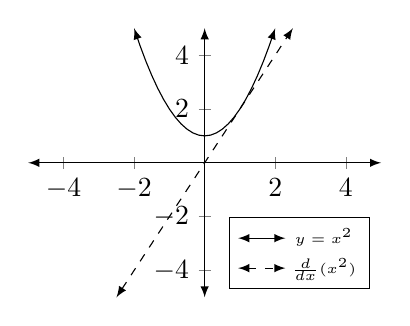
\begin{tikzpicture}
		\begin{axis}[plot,xmin=-5,xmax=5,ymin=-5,ymax=5]
			\addplot[mark = ,domain=-2:2, <->, >=latex]{x^2 + 1};
			\addlegendentry{$y=x^2$}
			\addplot[mark= , domain=-2.5:2.5, <->, >=latex, dashed]{2*x};
			\addlegendentry{$\ddx(x^2)$}
		\end{axis}
	\end{tikzpicture}
  \caption{Graph of $y=x^2$ and it's Derivative}
\end{figure}

The derivative is notated in many ways, the most common being $\ddx$. Be careful that you don't confuse the fraction-like syntax for division. While in some examples it \emph{can} behave as addition, in our case it does not. Another way that the derivative is often notated is by making a function prime. For example, if we have a function $f(x)$, then $f'(x)$ would represent it's respective derivative.

For this chapter you need to know the following derivative rules. If you already know them you can safely skip to the end of this section. \\

\begin{center}
	\vspace{-1cm}
	\begin{minipage}[b]{0.31\textwidth}
		\[\ddx(\e^x) = e^xdx\]
	\end{minipage}\hfill
	\begin{minipage}[b]{0.37\textwidth}
		\[\ddx(f(g(x))) = g'(x)f'(g(x))\]
	\end{minipage}\hfill
	\begin{minipage}[b]{0.31\textwidth}
		\[\ddx(x^a) = ax^{a-1}dx\]
	\end{minipage}
\end{center}

I will not go into the details of proving these derivatives. Very good explanations are available the Internet from reputable sources such as Khan Academy\footnote{\texttt{https://www.khanacademy.org/math/ap-calculus-ab/basic-differentiation-ab}}.
\subsection{Matrices and Vectors}
You may have noticed that the input data used in the first example looked an awful lot like a \emph{matrix} of numbers. A matrix is a grid of numbers that describes something. In our case, each row of the matrix described the input values that we put into our neural network. Matrices (plural for matrix) are notated by capital letters accompanied by a subscript describing the size of the matrix. For example,

\[
	A_{1\times2} =
	\begin{bmatrix}
		1 \\
		0 \\
	\end{bmatrix}
\]

As you can see, the subscript describes the size of the matrix much as you would notate a coordinate on the coordinate plane. It describes the number of columns (the $x$ dimension in coordinate terms) and then the number of rows (the $y$ dimension, in coordinate terms). Therefore, even if $A$ was not accompanied by a matrix showing actual numbers, the reader could understand that $A_{1\times2}$ Represents a matrix with 1 column and 2 rows.

\subsection{The Dot Product}

Machine learning is composed almost entirely of matrices and their close cousin, the vector (best described as a $1\times n$ matrix). A dot product can be used to multiply two  vectors together. For example;

\[
	\begin{bmatrix}
		a_1    \\
		a_2    \\
		\vdots \\
		a_n
	\end{bmatrix}
	\cdot
	\begin{bmatrix}
		b_1    \\
		b_2    \\
		\vdots \\
		b_n
	\end{bmatrix}
	= a_1b_1 + a_2b_2+ \dots +a_nb_n
\] %TODO Cite Khan Academy
\subsection{The Transpose}
The Transpose is another linear algebra function that manipulates matrices\footnote{Plural for Matrix}. However, instead of multiplying, dividing, adding, or subtracting, the Transpose serves to flip a matrix on it's side. For example, if $A$ represents an $m \times n$ matrix the transpose of $A$ is an $n \times m$ matrix. The transpose of a matrix is represented by superscript $\intercal$ on the variable representing the matrix. In our previous example, if $A$ is an $m \times n$ matrix then $A^\intercal$ is an $n \times m$ matrix.
\[
	\begin{align}
		A =
		\begin{bmatrix}
		_1a_1  & _2a_1  & \dots  & _ma_1  \\
		_1a_2  & _2a_2  & \dots  & _ma_2  \\
		\vdots & \vdots & \ddots & \vdots \\
		_1a_n  & _2a_n  & \dots  & _ma_n  \\
		\end{bmatrix} \\
		A^\intercal =
		\begin{bmatrix}
		_1a_1  & _1a_2  & \dots  & _1a_n  \\
		_2a_1  & _2a_2  & \dots  & _2a_n  \\
		\vdots & \vdots & \ddots & \vdots \\
		_ma_1  & _ma_2  & \dots  & _ma_n  \\
		\end{bmatrix}
	\end{align}\]
	\section{Algorithms}
	The algorithm used in the neural network built in this chapter is called the perceptron. Invented in 1958 at the Cornell Aeronautical Laboratory by a psychologist named Frank Rosenblatt\footcite{perceptronSrc}.
	First published in \emph{Psychological Review} under the title ``The Perceptron: A Probabilistic Model for Information Storage and Organization in the Brain'', the idea, although promising at first, proved unsuitable for classifying more than simple problems. This led to the study of Neural Networks being abandoned for several years, until the discovery of the multi-layer perceptron and it's capabilities (see chapter two for further info).

	The perceptron operates by taking the dot product of a set of inputs and a set of weights, and then running the result through a sigmoid function. In this case the weights are simply a set of numbers that are tuned to return a certain output when given certain inputs.

	The way this algorithm learns is called \emph{supervised learning}. This means that we feed it training data where each piece of input data is also labeled with a desired output data point. This differs from other methods of learning in that someone has to go through and label all of the data used to train the network before it can be used.

	The network is trained based on the following steps. All that the training process does is calculate the proper weights to apply to the input data.

	\begin{enumerate}
		\item Initialize Weights to Random Number\footcite{perceptron}.
		\item Pick Learning Weight between zero and one.
		\item For many iterations (More iterations returns more accurate weights but is also slower)%\footfullcite{perceptron}
		      \begin{enumerate}
		      	\item Make a prediction based on the training input and the weights
		      	\item Calculate the difference between the output value of the algorithm and the output value attached to the input data. This is called the error.
		      	\item Calculate an adjustment value for the weights by multiplying the error by the derivative of the sigmoid function for these data points
		      	\item Adjust the weights according to the product of the inputs and the adjustment value
		      \end{enumerate}
	\end{enumerate}

	The neural network that we build in this chapter is known as a single layer feed forward neural network with back-propagation. That's a mouthful at first, so let's break it down into parts to better understand it.

	\begin{itemize}
		\item \textbf{Single Layer:} This neural network consists of one layer of inputs that do calculation
		\item \textbf{Feed Forward:} Data is fed forward through the network and modified by weights
		\item \textbf{Neural Network:} Data is manipulated by a network of neurons.
		\item \textbf{Back-propagation:} The weights that manipulate the data are modified by looking at the output data and comparing it to the desired output.
	\end{itemize}

	For the more visually minded, the diagram below represents the neural network where $i_1, i_2, i_3$ are inputs, $w_1, w_2, w_3$ are weights that modify the inputs, and $o_1$ is the output.
	\begin{figure}[h]
		\centering
		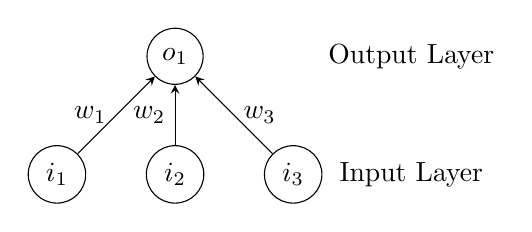
\begin{tikzpicture}[node distance = 1.5cm]
			%--Input Neurons--%
			\node(in1)[neuron]{$i_1$};
			\node(in2)[neuron,right of=in1]{$i_2$};
			\node(in3)[neuron,right of=in2]{$i_3$};

			%--Ouput Neuron--%
			\node(out1)[neuron,above of=in2]{$o_1$};

			%--Synapses--%
			\draw[arrow] (in1) -- node[anchor = east]{$w_1$} (out1);
			\draw[arrow] (in2) -- node[anchor = east]{$w_2$} (out1);
			\draw[arrow] (in3) -- node[anchor = west]{$w_3$} (out1);

			%--Other Labels--%
			\node(lay1)[right of=in3]{Input Layer};
			\node(lay2)[above of=lay1]{Output Layer};
		\end{tikzpicture}
    \caption{A Diagram Representing the Layout of the Neural Network}

	\end{figure}
	\clearpage
	\section{Code}
	The code for this book is written in Java. However, the sources used have code written in python. I chose Java because I find that python automates things too much to achieve a full understanding of what is actually going on behind the scenes.

	I don't start off writing this Neural Net by diving straight in and writing the perceptron itself. Instead I start off by writing some helper methods to handle the linear algebra, sigmoid curves, etc. If you want to see a full code listing see the end of this section.

	\subsection{Dot Product}
	To begin with I wrote a function that calculates the dot product of two $1\times n$ vectors. The function accepts two single dimensional arrays and returns the dot product of them. The code is as follows:
	\begin{lstlisting}[caption={Method to Calculate Dot Product in Java}]
public double dot(double[] input, double[] weight) {// Dot product of two 1xN arrays
	double sum = 0; //Define a variable that will hold the sum of the function
	for (int i = 0; i < input.length; i++) { //Repeat over the length of the input arrays
		sum += input[i] * weight[i]; //Add to the sum the product of the corresponding data points from each array
	}
	return sum; //Return the sum as the output of the method
}
// Overloaded method to accept integer as input
public double dot(int[] input, double[] weight){
    double[] out = new double[input.length];//Define output array
	for(int i = 0; i < input.length; i++){ //Convert input array from integer type to double type
		out[i] = input[i];
	}
    return dot(out,weight); //Run the dot function with the new input array
}
	\end{lstlisting}

	All that this code does is iterate over each array and sum the product of each item together. This process can be represented mathematically by the following:
	\[
		A =
		\begin{bmatrix}
			a_1    \\
			a_2    \\
			\vdots \\
			a_n    \\
		\end{bmatrix}
		B =
		\begin{bmatrix}
			b_1    \\
			b_2    \\
			\vdots \\
			b_n    \\
		\end{bmatrix}
	\]
	\[
		A \cdot B = \sum^n_{i=1} a_ib_i = a_1b_1 + a_2b_2 + \dots + a_nb_n
	\]
	Don't worry if this math looks confusing. All it's describing is the addition of all of the products of the matrices $A$ and $B$
	\subsection{Transpose}

	After the dot product code I wrote another method to calculate the transpose of a matrix (in programming just a multidimensional array). The code looks as follows:
	\begin{lstlisting}[caption = {Method to Return Transpose of an Array in Java}]
// Returns Transpose of  array
public int[][] transpose(int[][] in) { //Take input as array of integers
	int[][] out = new int[in[0].length][in.length]; //Create an output array using the dimensions of the input array, except flipped.
	// Set out[x][y] equal to input[y][x]
	for (int y = 0; y < in.length; y++) {
		for (int x = 0; x < in[0].length; x++) {
			out[x][y] = in[y][x];
		}
	}
	return out; //Return output array as the output of the method
}
	\end{lstlisting}

	Much like the dot product code from before, this code iterates over an array using a \lstinline{for} loop, except that this time instead of taking the products of each item and then summing them this just assigns each value to a new matrix such that:
	\[
		_na_m \rightarrow {}_mb_n
	\]

	\printbibliography
\end{document}
